\documentclass[a4paper,12pt]{article} 

%%% Работа с русским языком
\usepackage{cmap}                           % поиск в PDF
\usepackage{mathtext} 			 	       % русские буквы в формулах
\usepackage[T2A]{fontenc}               % кодировка
\usepackage[utf8]{inputenc}              % кодировка исходного текста
\usepackage[english,russian]{babel}  % локализация и переносы
\usepackage{wrapfig}
\usepackage{gensymb}
\usepackage{textcomp}
\usepackage{multirow}
\usepackage{amsmath,amsfonts,amssymb,amsthm,mathtools} % AMS
\usepackage{euscript}	 % Шрифт Евклид
\usepackage{mathrsfs} % Красивый матшрифт
\usepackage{graphicx}%Вставка картинок правильная
\usepackage{float}%"Плавающие" картинки
\usepackage{wrapfig}%Обтекание фигур (таблиц, картинок и прочего)
\title{Лабораторная работа 2.2.1 

Исследование взаимной диффузии газов}
\author{Кагарманов Радмир Б01-106}
\date{17 мая 2022 г.}
\begin{document}

\maketitle
\thispagestyle{empty}
\newpage
\setcounter{page}{1}
\paragraph{Цель работы:} исследовать взаимную диффузию двух газов.
\paragraph{В работе используется:} два сосуда объёмами $V_1$ и $V_2$, соединённые трубкой длиной $L$ и сечения $S$; система откачки и напуска воздуха и гелия; форвауумный насос; манометр.

\paragraph{Теоретические сведения\\} Диффузией называют самопроизвольное взаимное проникновение веществ друг в друга, происходящее вследствие хаотичного теплового движения молекул. \\
Диффузия в системе, состоящей из двух компонентов a и b (бинарная
смесь), подчиняется закону Фика. Перемешивание газов в работе можно приближенно описывать как диффузию примеси лёгких частиц He на практически стационарном фоне воздуха. Коэффициент диффузии в таком приближении равен:
\begin{equation}
    D=\frac{1}{3}\lambda \bar v,
\end{equation}
где $\bar v=\sqrt{\frac{8RT}{\pi \mu}}$ - средняя тепловая скорость частиц примеси, $\lambda = \frac{1}{n_0 \sigma}$ - их длина свободного пробега, $n_0$ - концентрация рассеивающих центров(фона), $\sigma$ - сечение столкновения частиц примеси с частицами фона.\\
Для бинарной смеси формула (1) сохраняется, если 1) под $\lambda$ понимать величину $\lambda = \frac{1}{n_{\sum} \sigma}$, где $n_{\sum} = n_{\text{He}} + n_{\text{В}} = \frac{P}{k_{Б} T}$ - полная концентрация частиц и 2) под $\bar v$ понимать среднюю относительную скорость скорость частиц разных сортов. \\
Таким образом, теория предсказывает, что коэффициент диффузии бинарной смеси обратно пропорционален давлению в системе $D\propto \frac{1}{P}$.\\
Разность концентраций будет убывать по экспоненциальному закону:
\begin{equation}
    \Delta n=\Delta n_0 e^{-\frac{t}{\tau}},
\end{equation}
где $\tau=\frac{1}{D}\frac{VL}{2S}$.\\
В процессе
диффузии разность концентраций убывает по закону (2), и по тому
же закону изменяется напряжение:
\begin{equation}
    U=U_0 e^{-\frac{t}{\tau}}
\end{equation}

\paragraph{Установка\\}
\begin{figure}[!h]
\centering
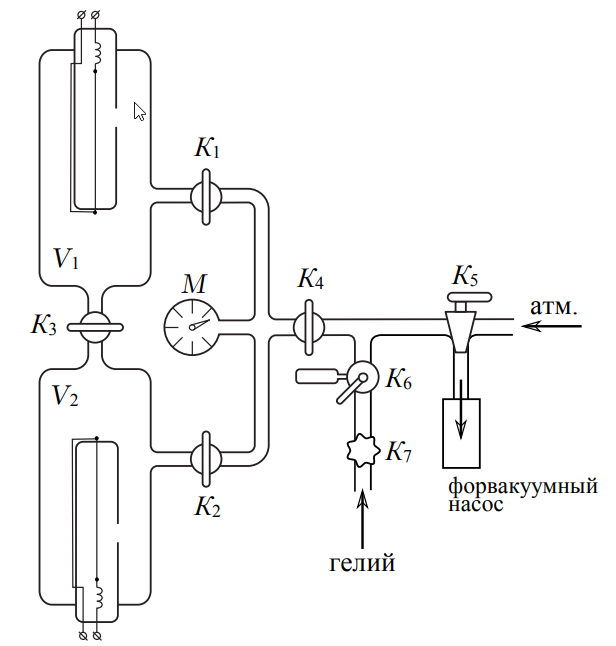
\includegraphics[width=0.6\linewidth]{Установка.png}
\caption{Экспериментальная установка}
\label{fig:mpr}
\end{figure}
Измерительная часть установки состоит из двух сосудов $V_1$ и $V_2$, размещённых вертикально. Краны $K_1$ и $K_2$ служат для управления откачкой и
подачей воздуха/гелия в сосуды. Диффузия осуществляется через тонкую
короткую трубку, соединяющую сосуды, оснащённую краном $K_3$. К соединительным трубкам подключен манометр $M$, измеряющий разность давлений между соединительными трубками и атмосферой, и позволяющий
измерять давления в разных частях системы (в зависимости от положения
кранов).
\newpage
\paragraph{Обработка результатов\\}
\subparagraph{1.} Построим график зависимости $ln ~U$ от $t$, чтобы по формулам (3) и $\tau=\frac{1}{D}\frac{VL}{2S}$ найти $D$ для каждого эксперимента.
\begin{figure}[!h]
\centering
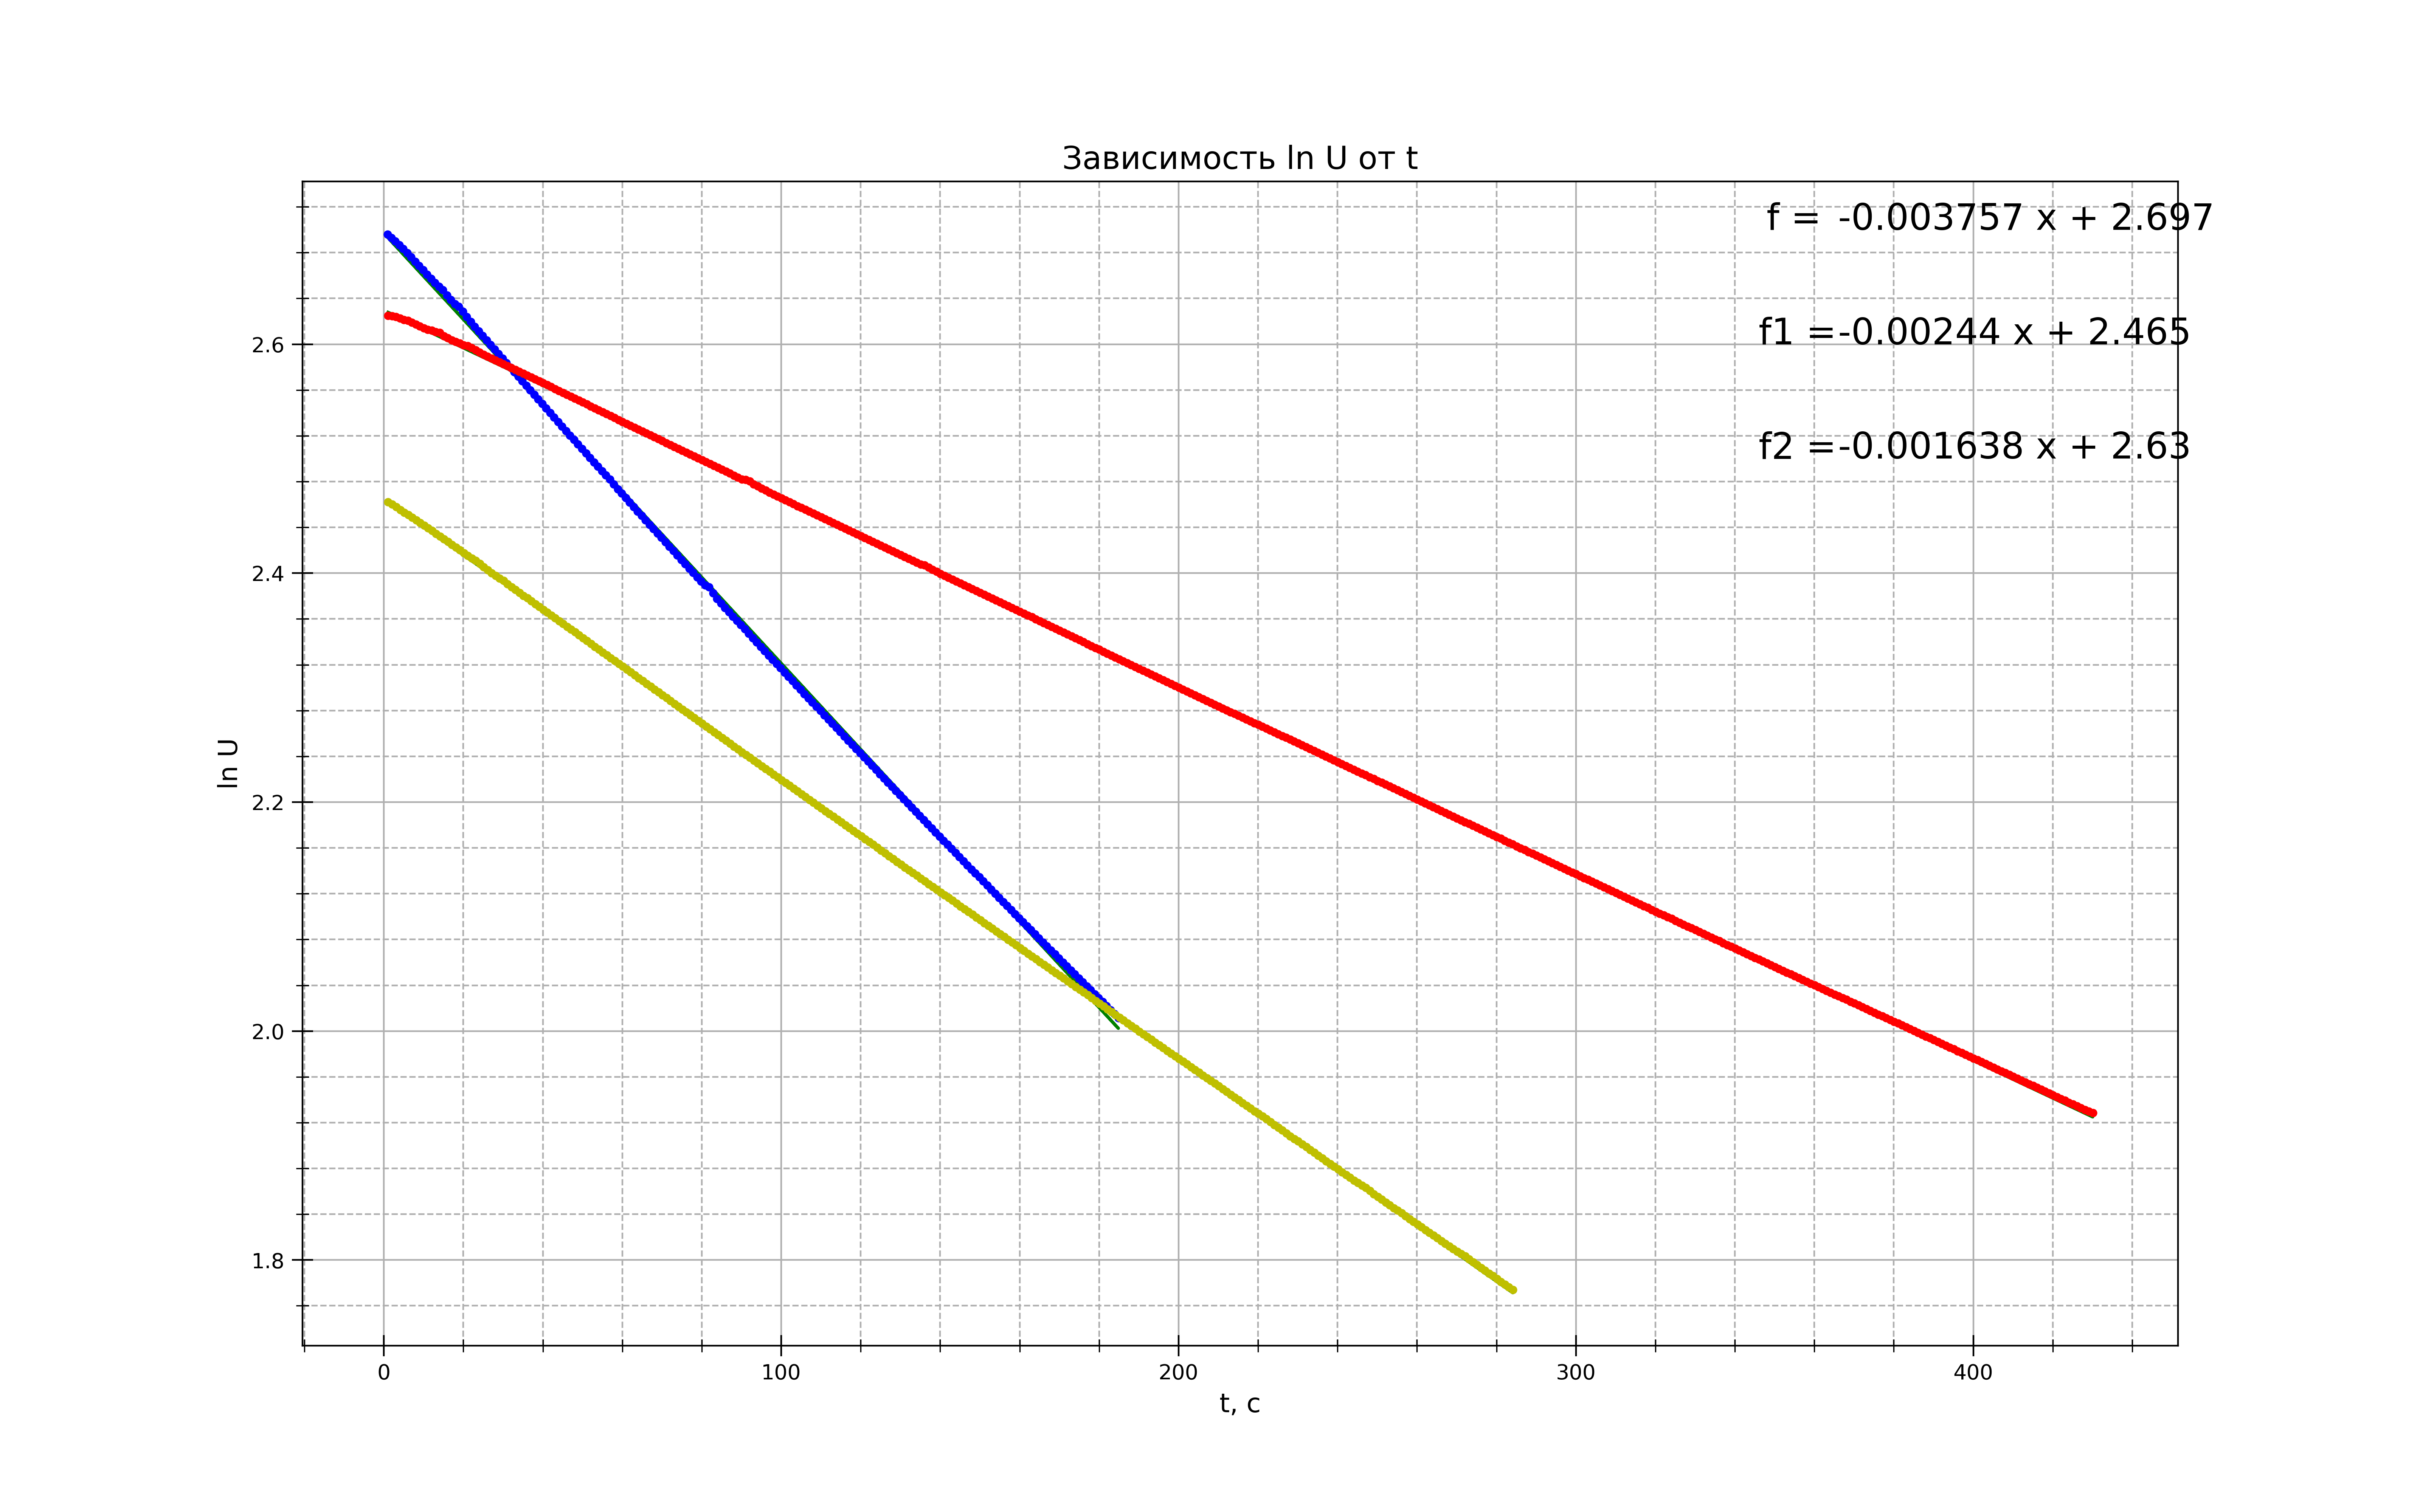
\includegraphics[width=0.8\linewidth]{U(t)1.png}
\caption{Графики зависимости $ln ~U$ от $t$}
\label{fig:mpr}
\end{figure}
Коэффициент диффузии рассчитывается по формуле $D = -\frac{kVL}{2S}$, его ошибка будет составлять $\sigma_D = D\sqrt{(\frac{\sigma_V}{V})^2+(\frac{\sigma_k}{k})^2+(\frac{\sigma_{L/S}}{L/S})^2}$

Параметры установки: $V = 420 \pm 10 ~см^3$, $L/S = (9,0 \pm 0,1)~ \frac{1}{см}$.
\begin{center}
    $P_1 = 41,47 ~торр: ~ D_1=7,10\pm 0,19~ \frac{см^{2}}{с}$\\
    $P_2 = 82,94 ~торр: ~ D_1=4,61\pm 0,12~ \frac{см^{2}}{с}$\\
    $P_3 = 120,64 ~торр: ~ D_1=3,10\pm 0,08~ \frac{см^{2}}{с}$
\end{center}
\newpage
\subparagraph{2.} На Рис. 3 изображена зависимость $D(\frac{1}{P})$. С её помощью мы найдём коэффициент диффузии при атмосферном давлении.
\begin{figure}[!h]
\centering
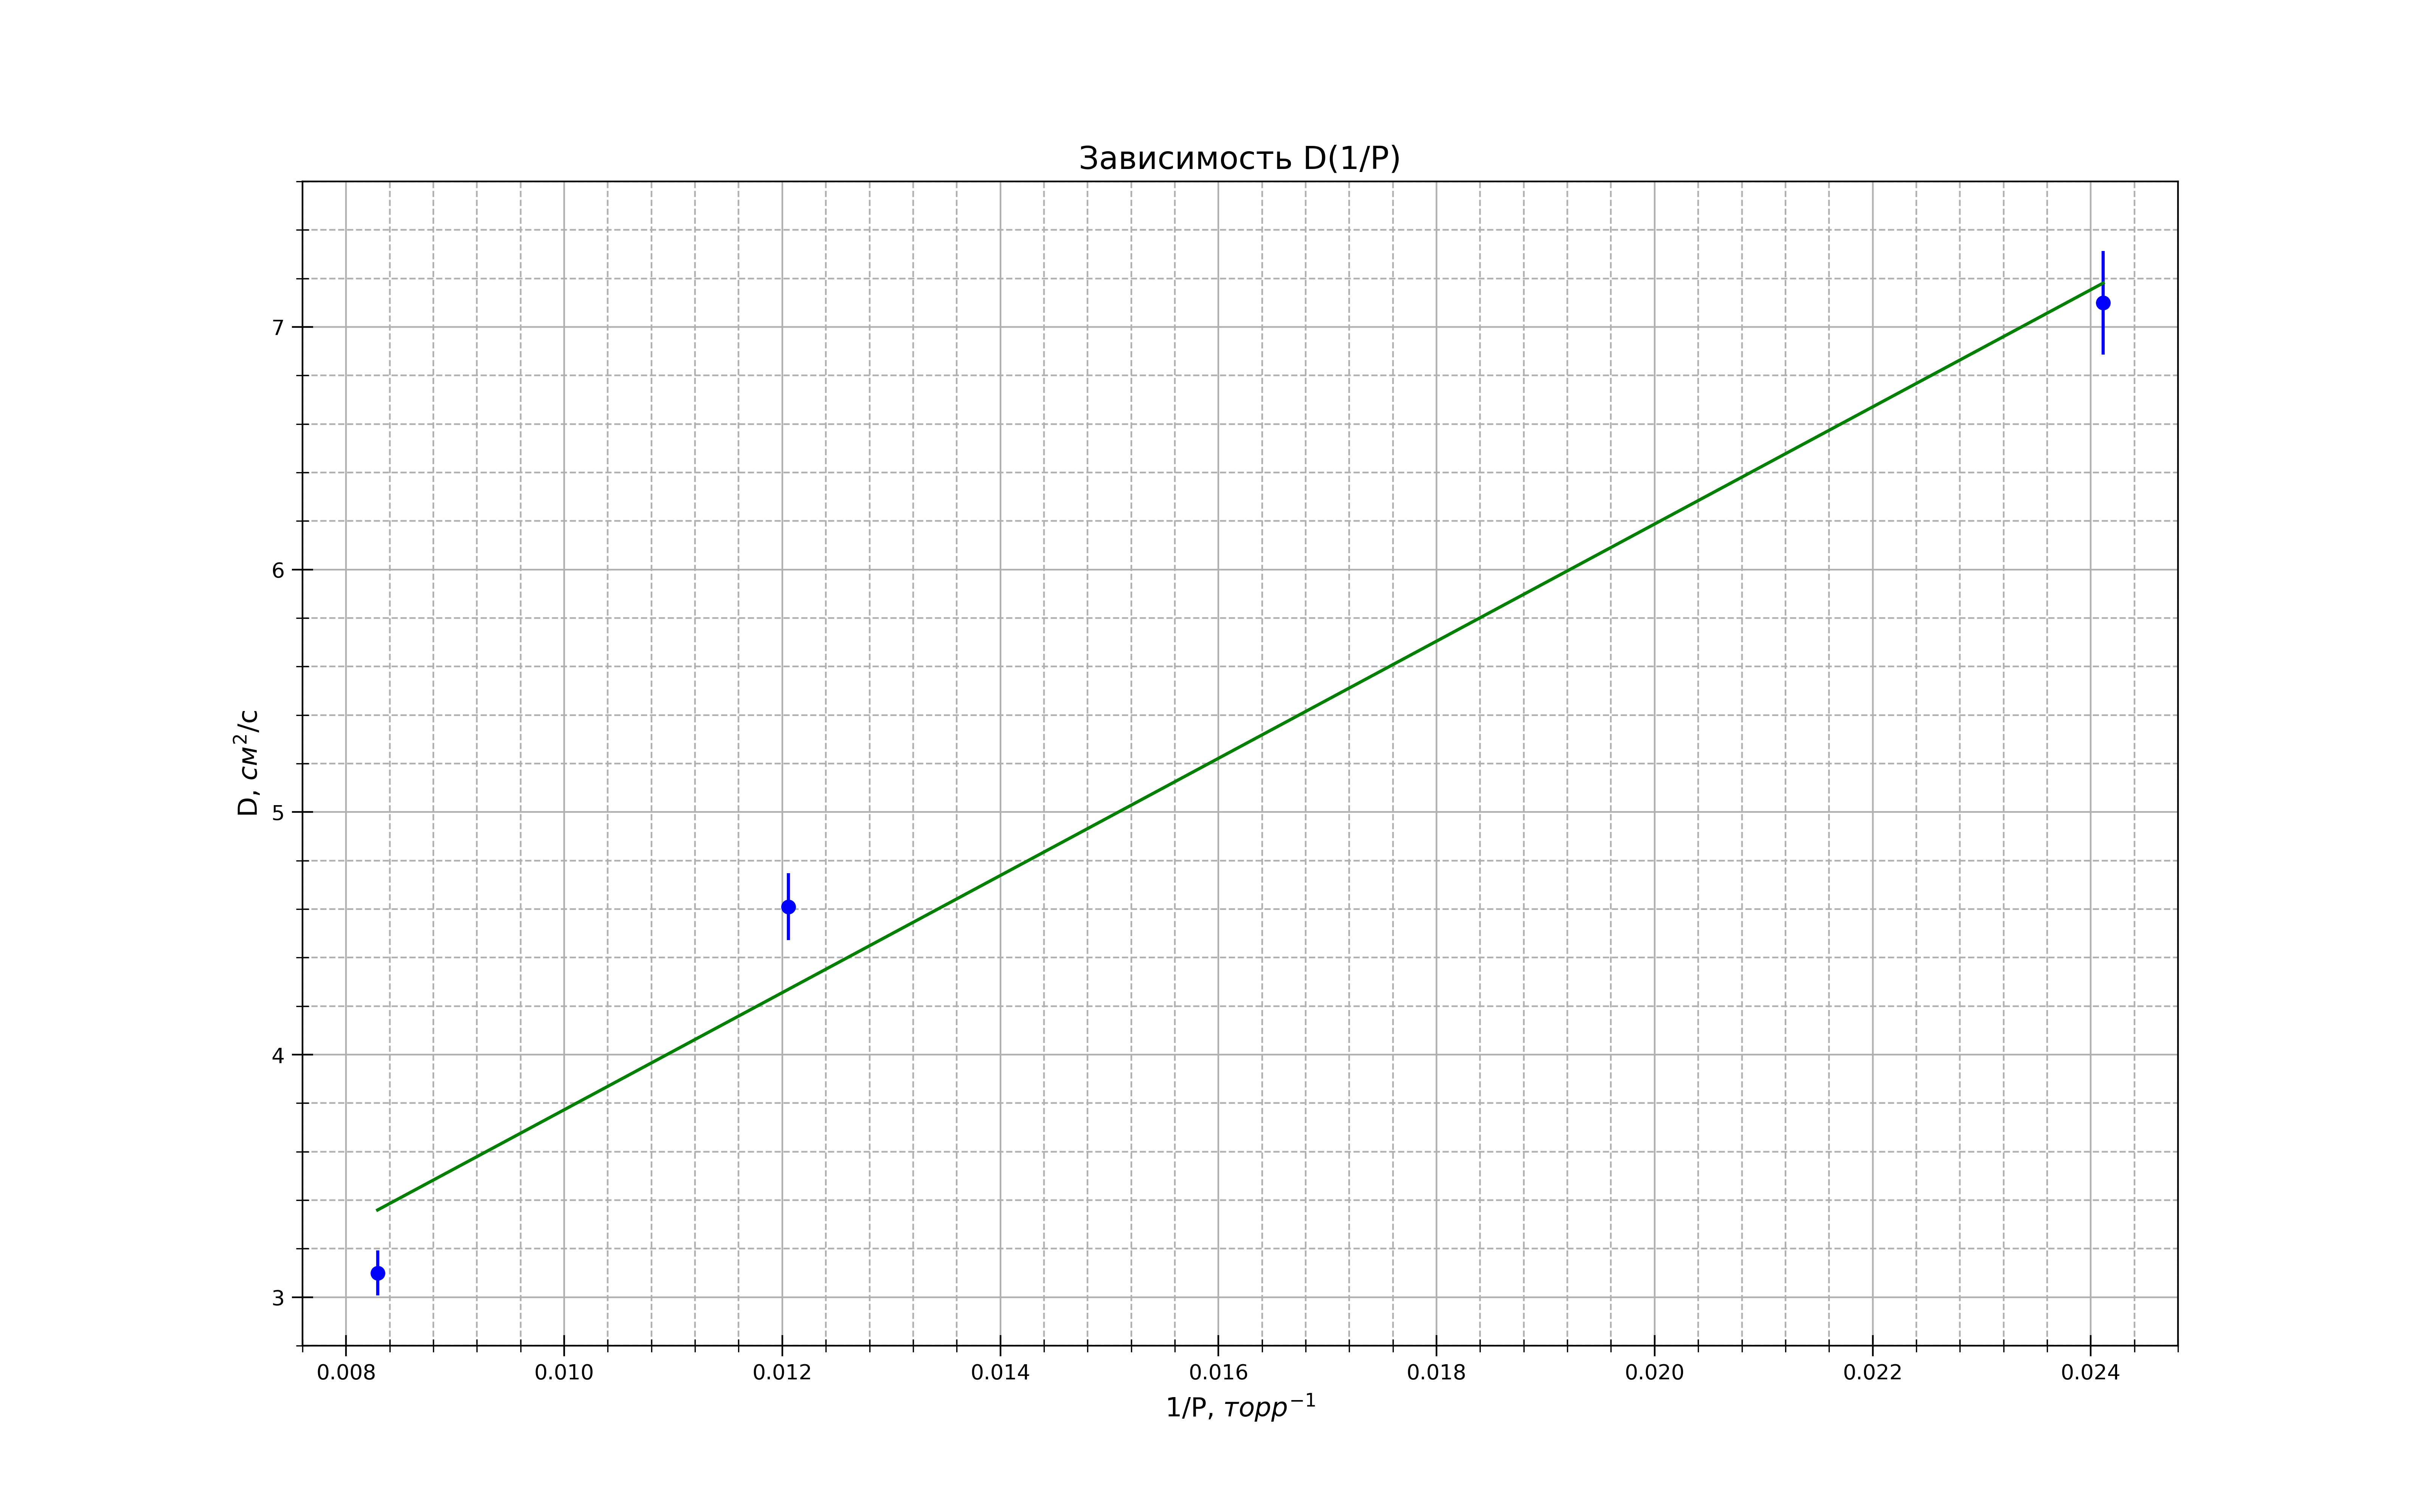
\includegraphics[width=0.8\linewidth]{D(P).png}
\caption{График зависимости $D(\frac{1}{P})$}
\label{fig:mpr}
\end{figure}
\begin{center}
    $D_{а}=0,675\pm 0,061~ \frac{см^{2}}{c}$
\end{center}
\subparagraph{3.} Оценим длину свободного пробега молекулы по формуле:
\begin{center}
$\lambda = 3D \sqrt{\frac{\pi \mu }{8RT}}$
\end{center}
Возьмём температуру $296~ K$. Тогда $\lambda=162$ нм.

Оценим эффективное сечение столконевний атомов гелия с частицами воздуха при температуре 299 К и давлении $10^5$ Па:

\begin{center}
$\sigma = \frac{1}{\lambda n}$\\
$\sigma = \frac{kT}{\lambda P} = 2,5 \cdot 10^{-19}~м^{2}$
\end{center}

\paragraph{Вывод:} в данной лабораторной работе мы исследовали взаимную диффузию воздуха и гелия. Были найдены длина свободного пробега атомов гелия в воздухе $\lambda=162~нм$ и эффективное сечение столкновений атомов гелия с воздухом $\sigma=2,5\cdot 10^{-19}~м^{2}$
\end{document}
